\chapter{\texorpdfstring{Orchestration e Collaboration}{Orchestration e Collaboration}}
\label{ch:06}
\lecturemeta{Lezione 06 \quad\textbullet\quad 2026-07-03 \quad\textbullet\quad Roberto Bruni}{Weske, \emph{Business Process Management}, Sect.1.1}

Finora abbiamo guardato un processo come qualcosa di isolato. Ma nella realtà i processi \emph{interagiscono}: un'azienda che vende deve coordinarsi con chi compra, e ciascuna ha la propria logica interna. Questa lezione affronta due temi. Primo, un nuovo linguaggio di modellazione, l'\textbf{EPC}, che affianca BPMN e workflow net. Secondo — ed è il cuore della lezione — i \textbf{tre punti di vista} da cui si può guardare un insieme di processi che collaborano: l'\textbf{orchestration} (uno solo che controlla), la \textbf{collaboration} (più attori che si scambiano messaggi) e la \textbf{choreography} (le regole globali dell'interazione).

\section{\texorpdfstring{EPC: Event-driven Process Chain}{EPC: Event-driven Process Chain}}

L'\textbf{EPC} è un linguaggio di tipo flow-chart nato all'inizio degli anni '90 come parte del framework \textbf{ARIS} (Architecture of Integrated Information Systems) di \textbf{Wilhelm-August Scheer}. È pensato per due usi concreti: configurare un'implementazione di ERP (Enterprise Resource Planning) e guidare la modellazione, analisi e ridisegno dei processi di business. Il suo punto di forza dichiarato è la \textbf{semplicità}: una notazione informale, minimale e intuitiva, che non richiede una "legenda" per essere capita. Ha anche un formato di interscambio in XML, l'\textbf{EPC Markup Language} (\texttt{.epml}).

\begin{boxdefinition}{Event-driven Process Chain (EPC)}
Un grafo \textbf{ordinato di eventi e funzioni}, dotato di connettori che permettono l'esecuzione alternativa e parallela dei processi, specificata tramite gli operatori logici \textbf{AND}, \textbf{OR} e \textbf{XOR}.
\end{boxdefinition}

L'EPC ha quattro tipi di ingredienti, ognuno con la sua forma grafica precisa.

\begin{figure}[!htb]
\centering
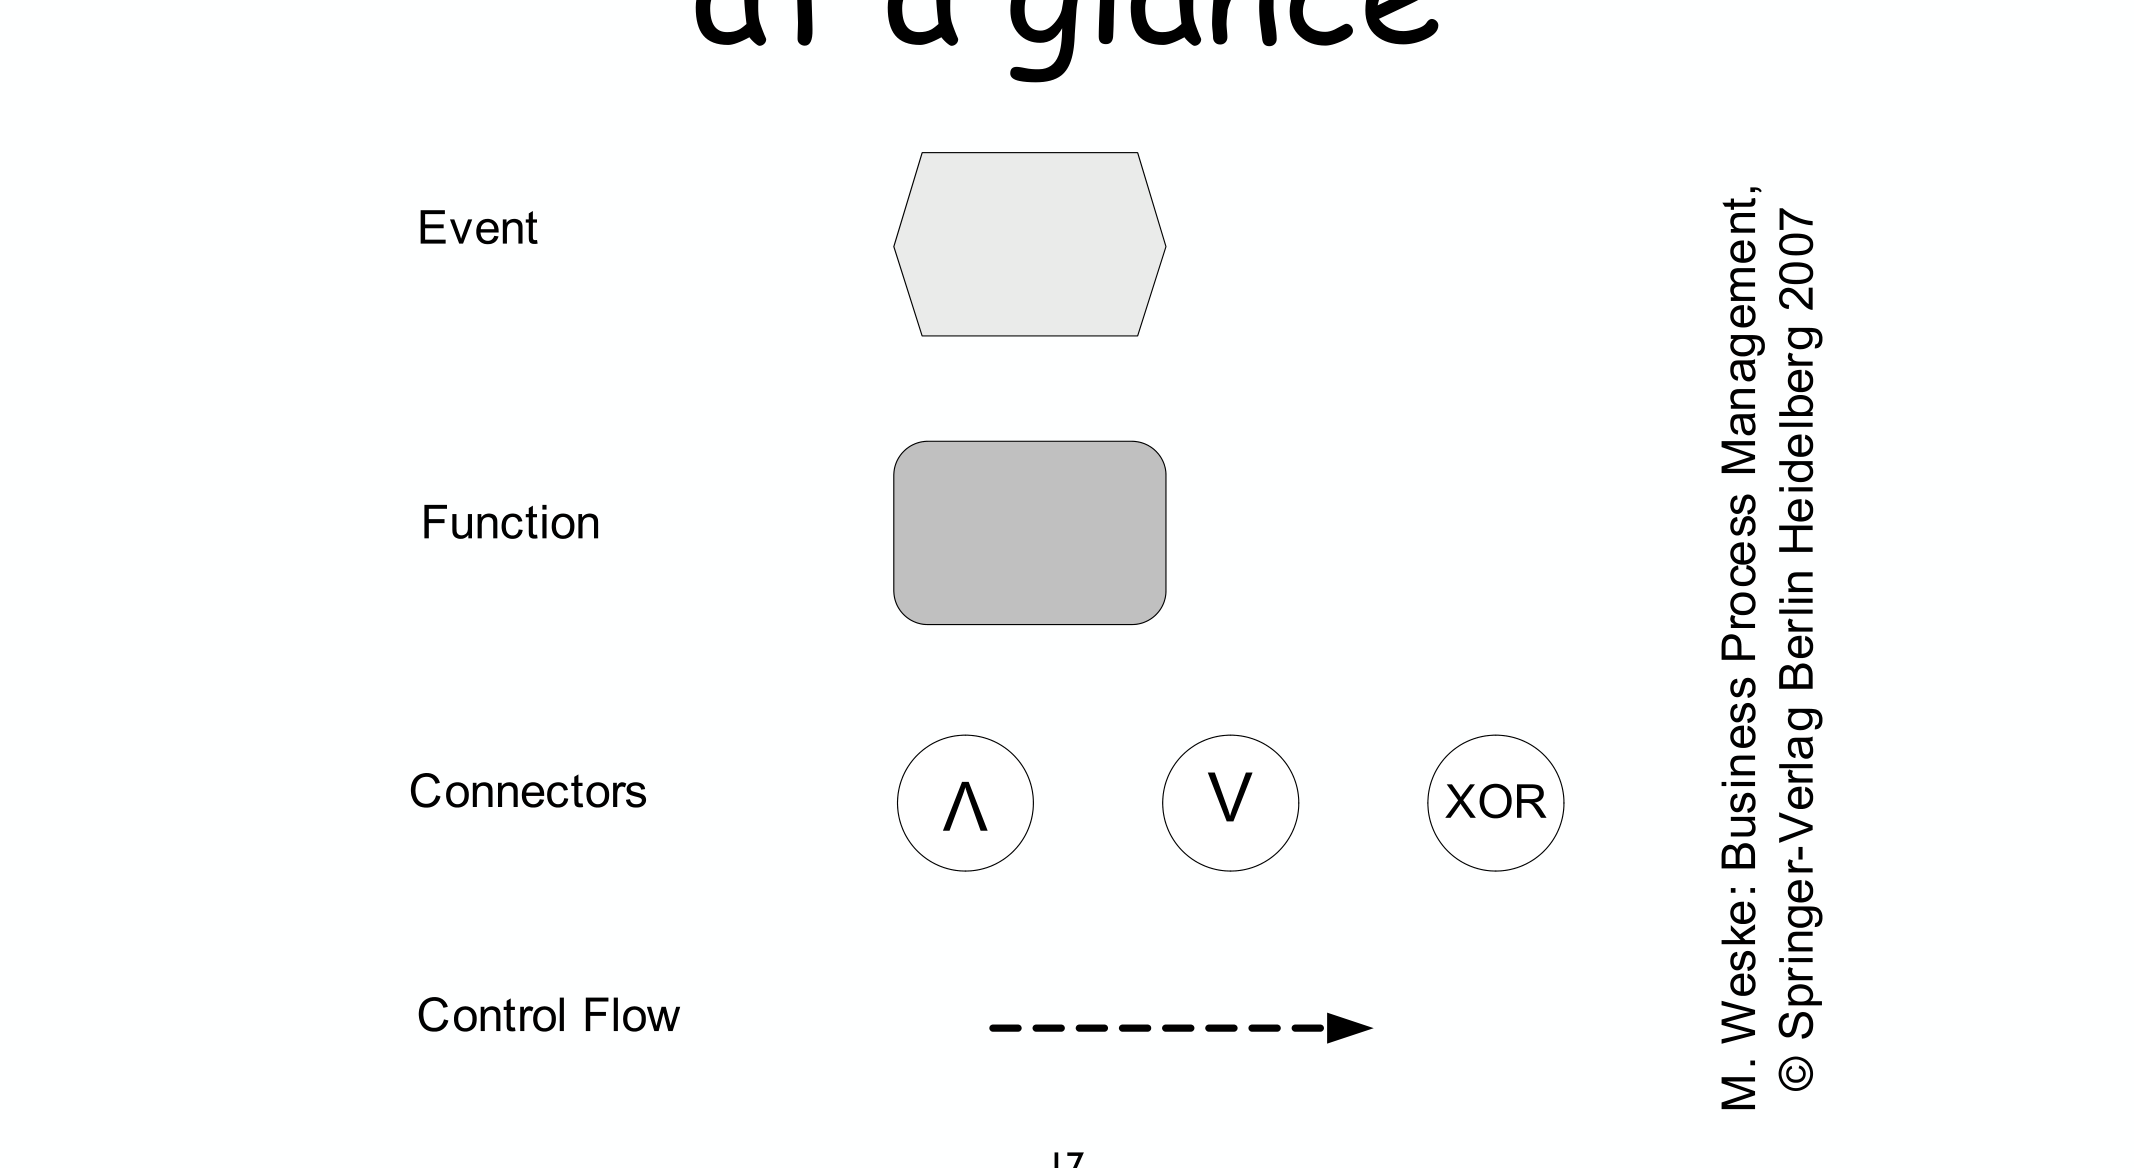
\includegraphics[width=0.74\linewidth,height=0.34\textheight,keepaspectratio]{images/06-orchestration_p16_epc-ingredients.png}
\caption{Gli ingredienti dell'EPC.}
\end{figure}

\begin{boxdefinition}{I quattro ingredienti dell'EPC}
\begin{itemize}
\item \textbf{Event} (esagono): un elemento \textbf{passivo} che descrive \emph{sotto quali circostanze} un processo (o una funzione) opera, o \emph{in quale stato} risulta — in pratica, pre- e post-condizioni. Ogni diagramma EPC deve \textbf{iniziare e finire con degli eventi}.
\item \textbf{Function} (rettangolo arrotondato): un elemento \textbf{attivo} che descrive un task o un'attività del processo. Una funzione può essere \textbf{raffinata} in un altro diagramma EPC (composizione gerarchica).
\item \textbf{Logical connector} (cerchio, a volte ottagono): esprime le relazioni logiche tra i rami di uno split o di un join. I tre operatori sono \textbf{AND} ($\wedge$), \textbf{OR} ($\vee$) e \textbf{XOR} ($\times$).
\item \textbf{Control flow} (freccia tratteggiata): collega eventi, funzioni e connettori, esprimendo dipendenze causali.
\end{itemize}
\end{boxdefinition}

Una regola strutturale caratteristica dell'EPC è l'\textbf{alternanza} tra eventi e funzioni lungo il flusso (un evento abilita una funzione, che produce un evento, e così via), esattamente come i Petri net alternano place e transition.

\begin{boxwarning}{La semantica dell'OR-join è insidiosa}
Mentre AND e XOR sono chiari, l'\textbf{OR-join} ha un significato sorprendentemente delicato. Quando su un ramo arriva un solo input, il join non può decidere subito: deve \textbf{aspettare l'altro input}, a meno che non sia \emph{garantito} che l'altro non arriverà mai. Questa è una condizione \textbf{non-locale} (dipende da cosa può ancora succedere altrove nella rete), ed è la ragione per cui la semantica formale dell'OR-join è notoriamente problematica.
\end{boxwarning}

\section{\texorpdfstring{I tre punti di vista sull'interazione tra processi}{I tre punti di vista sull'interazione tra processi}}

Veniamo al cuore della lezione. Quando più processi collaborano, possiamo modellarli da tre prospettive diverse. Non sono modelli in competizione: descrivono la \emph{stessa} realtà a livelli di astrazione differenti, e la scelta dipende da cosa vogliamo mettere in evidenza.

\subsection{\texorpdfstring{Orchestration: un unico punto di vista}{Orchestration: un unico punto di vista}}

Un business process, per definizione, è eseguito \textbf{da una singola organizzazione}. Perciò l'ordine delle sue attività può essere controllato in modo \textbf{centralizzato} da un componente software (il BPMS) gestito da quell'organizzazione. Questo tipo di controllo si chiama \textbf{orchestration}.

\begin{boxdefinition}{Orchestration}
Un modello a \textbf{singolo punto di vista} (single viewpoint), in cui un agente centrale controlla l'ordine delle attività di \emph{un} processo. L'analogia è con il \textbf{direttore d'orchestra}, che dal centro coordina tutti i musicisti.
\end{boxdefinition}

\begin{figure}[!htb]
\centering
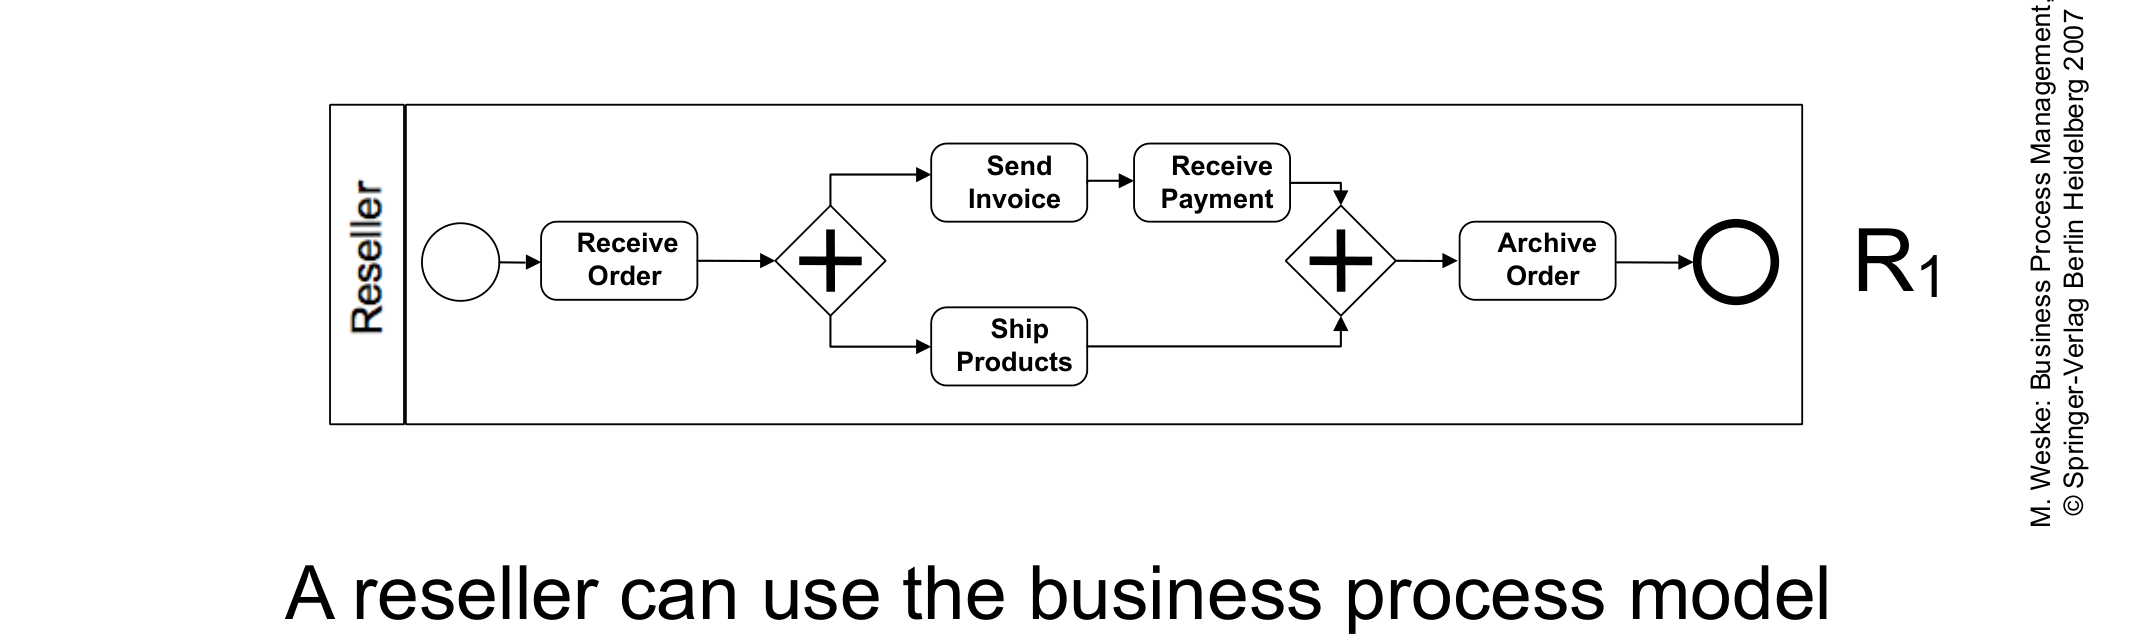
\includegraphics[width=0.74\linewidth,height=0.34\textheight,keepaspectratio]{images/06-orchestration_p31_reseller-orchestration.png}
\caption{Orchestration del reseller (R1) in BPMN. È un processo interno a una sola organizzazione: dopo aver ricevuto l'ordine, le attività di fatturazione/incasso e di spedizione avvengono \textbf{in parallelo} (gateway \texttt{+}). Il reseller usa questo modello per configurare il proprio BPMS, e tutte le istanze verranno eseguite come specificato.}
\end{figure}

\subsection{\texorpdfstring{Collaboration: più punti di vista che si scambiano messaggi}{Collaboration: più punti di vista che si scambiano messaggi}}

Se ora consideriamo \emph{insieme} il processo del reseller e quello del buyer, ciascuno resta autonomo e controllato dalla propria organizzazione, ma i due devono \textbf{comunicare}. Questo è il livello della \textbf{collaboration}.

\begin{boxdefinition}{Collaboration}
Un modello \textbf{decentralizzato a punti di vista multipli} (multiple viewpoints). Comprende le attività di \textbf{processi autonomi} e il modo in cui interagiscono per raggiungere un obiettivo comune. Ogni processo è eseguito da una sola organizzazione, ma processi cross-organizzativi possono interagire tra loro. Collegare le attività correlate di processi distinti è, appunto, la collaboration.
\end{boxdefinition}

Il meccanismo dell'interazione è lo \textbf{scambio di messaggi}: messaggi elettronici o oggetti fisici trasportati da un processo all'altro. Graficamente, in sintassi BPMN, il \textbf{message flow} si rappresenta con \textbf{archi tratteggiati} (distinti dalle frecce piene del control flow interno).

\begin{figure}[!htb]
\centering
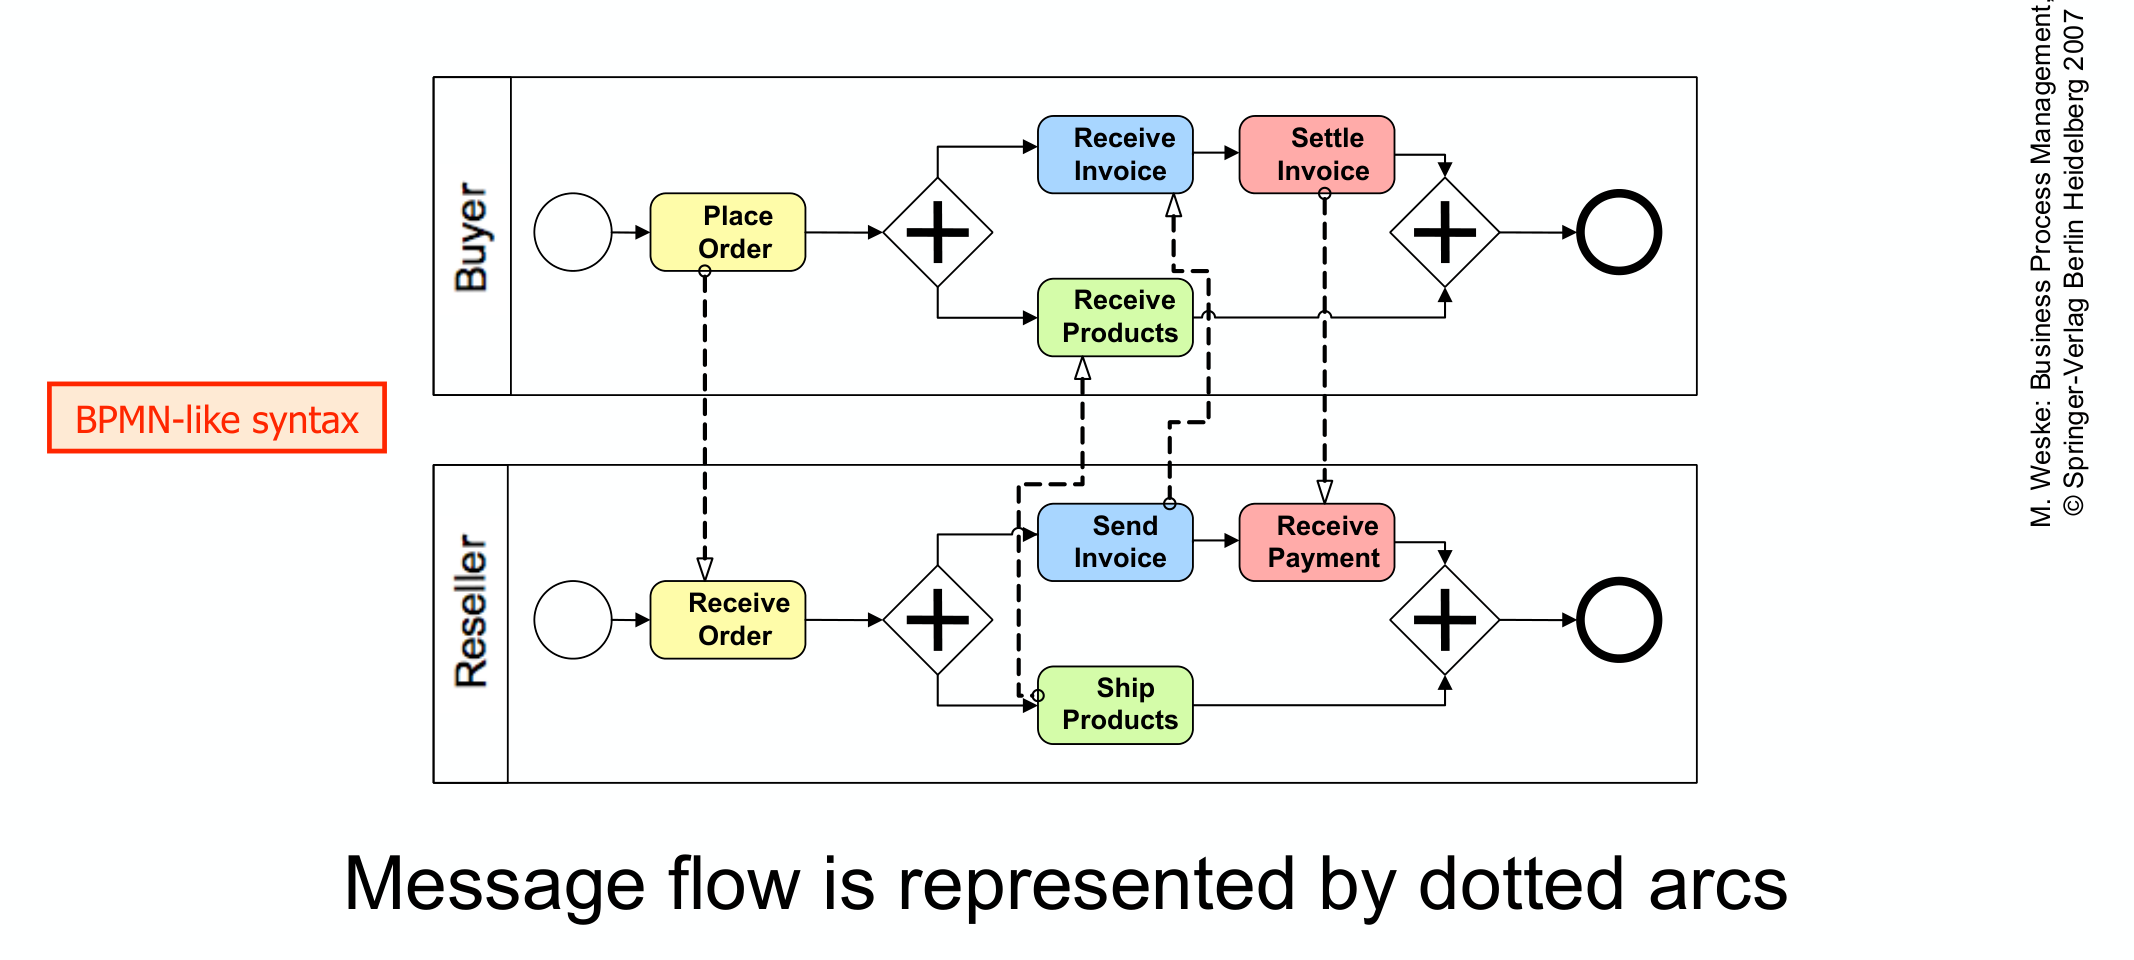
\includegraphics[width=0.74\linewidth,height=0.34\textheight,keepaspectratio]{images/06-orchestration_p35_collaboration.png}
\caption{Collaboration Buyer–Reseller. Ogni organizzazione ha la propria pool con il proprio control flow interno (frecce piene); gli \textbf{archi tratteggiati} tra le pool sono i \textbf{message flow} che collegano, per esempio, il "Place Order" del buyer al "Receive Order" del reseller.}
\end{figure}

\subsection{\texorpdfstring{Choreography: il punto di vista globale}{Choreography: il punto di vista globale}}

C'è infine un terzo livello, che astrae ancora di più: la \textbf{choreography}. Qui non ci interessa la logica interna di ciascun partecipante, ma \textbf{solo le interazioni} tra di loro, viste dall'esterno.

\begin{boxdefinition}{Choreography}
Un modello a \textbf{punto di vista globale} (global viewpoint) che specifica le interazioni di un insieme di processi. Si differenzia: - dall'\textbf{orchestration} perché \textbf{non c'è un agente centrale} che controlla le attività; - dalla \textbf{collaboration} perché contiene \textbf{solo le attività di interazione} tra i partecipanti, non la logica interna di ciascuno.

L'analogia è con i \textbf{ballerini} di una coreografia: si comportano in modo autonomo, ma seguono ciascuno la propria parte in una danza concordata.
\end{boxdefinition}

\begin{figure}[!htb]
\centering
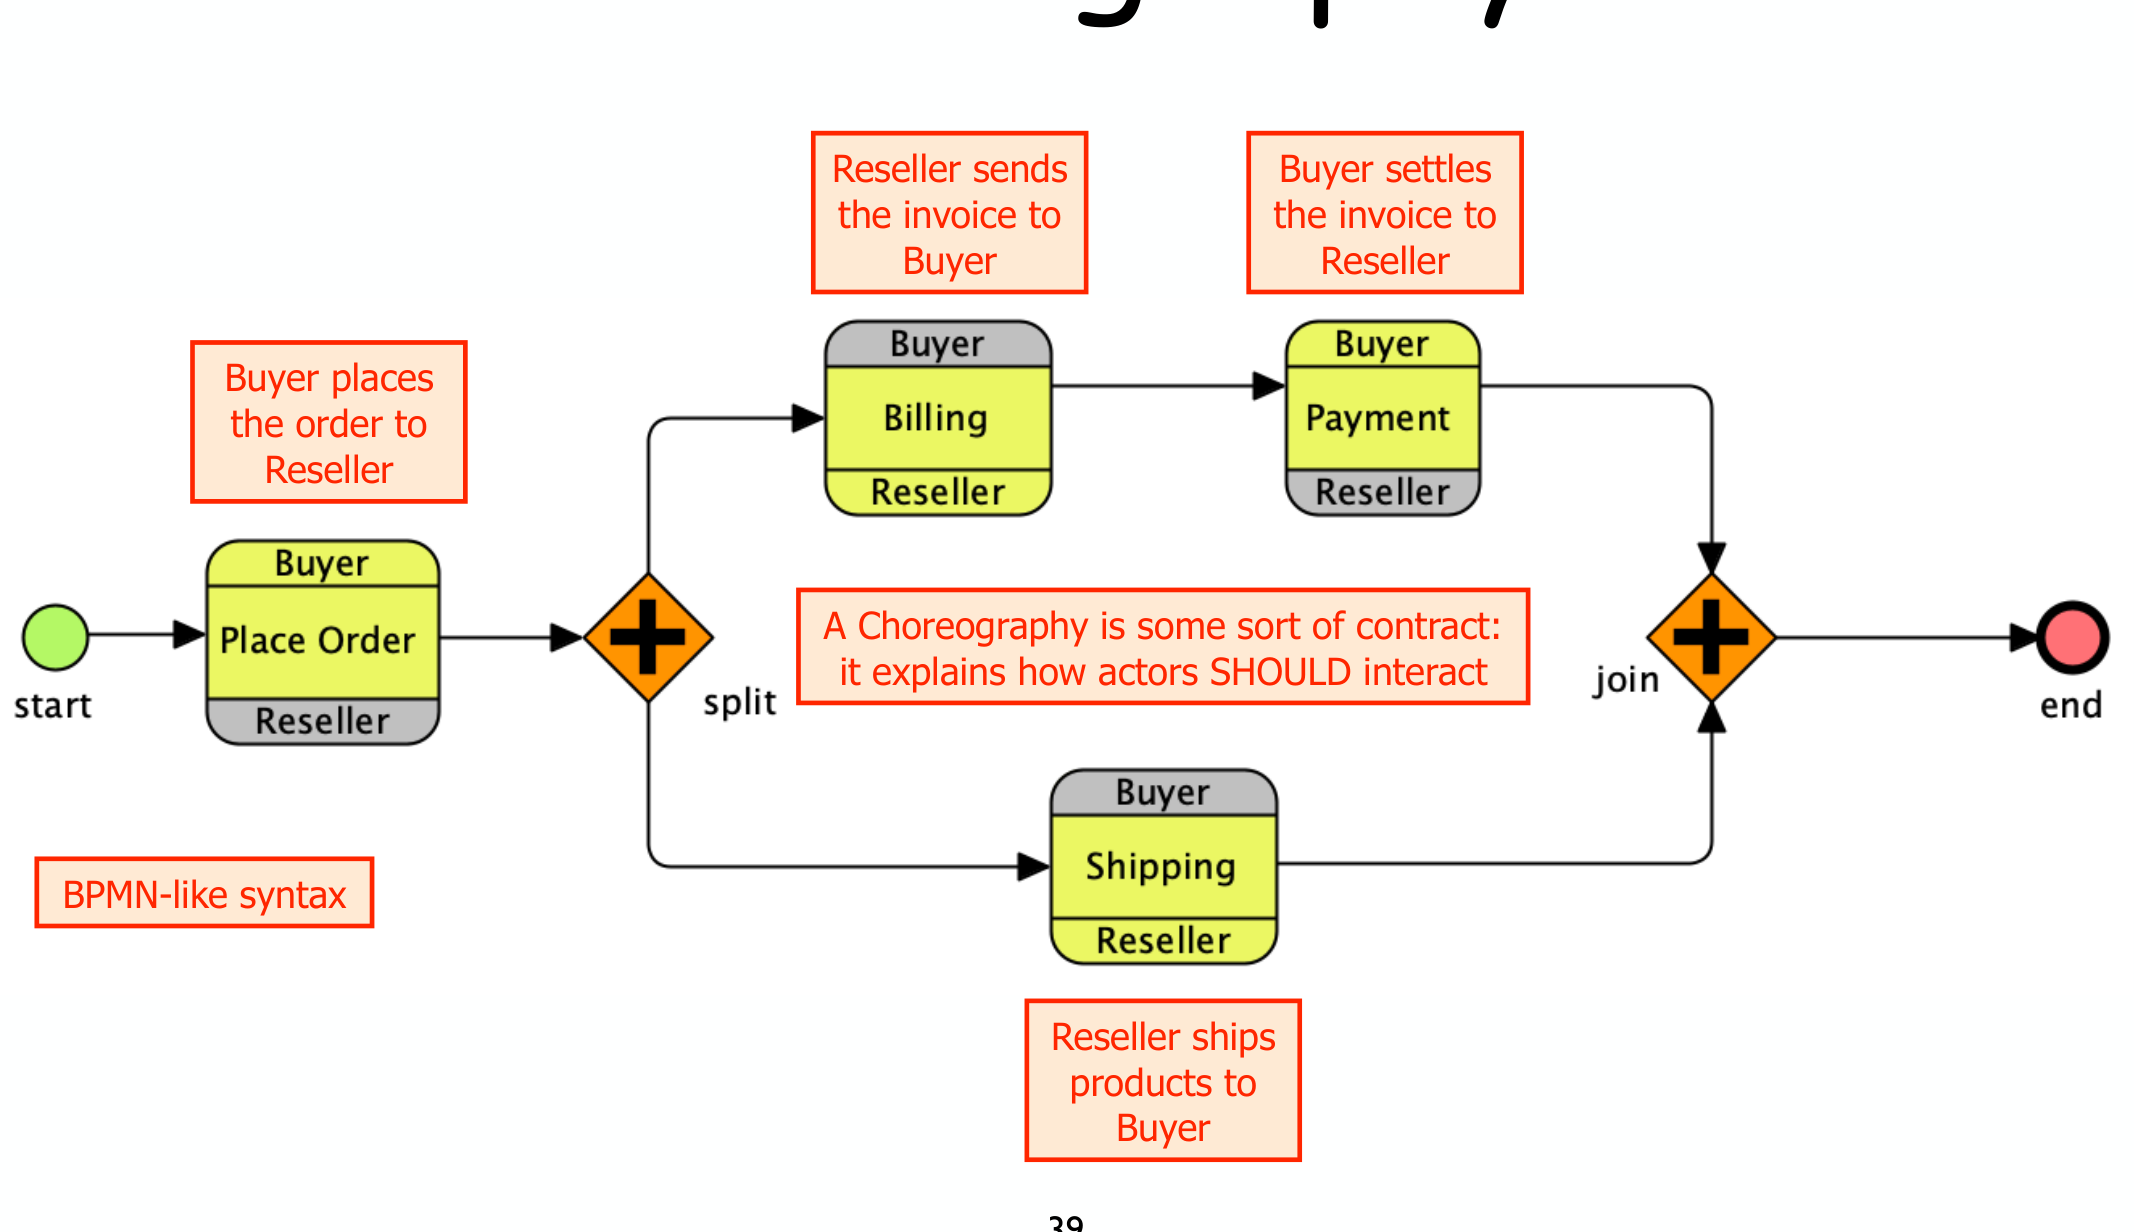
\includegraphics[width=0.74\linewidth,height=0.34\textheight,keepaspectratio]{images/06-orchestration_p38_choreography.png}
\caption{Choreography. Ogni box è un'\textbf{attività di interazione} con i due partecipanti (Buyer/Reseller) sulle bande; il diagramma dice, per esempio, "il Buyer piazza l'ordine al Reseller", "il Reseller spedisce i prodotti al Buyer". Una choreography è una sorta di \textbf{contratto}: dice come gli attori \textbf{dovrebbero} interagire, senza imporre come ciascuno realizza internamente la propria parte.}
\end{figure}

\begin{boxabstract}{I tre punti di vista a confronto}
\begin{itemize}
\item \textbf{Orchestration} — \emph{single viewpoint}: un attore centrale controlla; è il "dentro" di una singola organizzazione (direttore d'orchestra).
\item \textbf{Collaboration} — \emph{multiple viewpoints}: più attori autonomi con la loro logica interna, collegati da message flow (musicisti che si passano segnali).
\item \textbf{Choreography} — \emph{global viewpoint}: solo le regole d'interazione, nessun controllore centrale (ballerini che seguono la coreografia).
\end{itemize}
\end{boxabstract}

\section{\texorpdfstring{Compatibilità tra processi}{Compatibilità tra processi}}

C'è un problema pratico che emerge appena si mettono insieme processi \textbf{sviluppati separatamente}: non è affatto garantito che riescano a lavorare insieme. Ciascuno è stato progettato con le proprie assunzioni sull'ordine delle attività, e se queste assunzioni non combaciano l'interazione può \textbf{bloccarsi}.

Consideriamo un buyer B4 che si aspetta di \emph{ricevere i prodotti prima di pagare la fattura}, e un reseller R2 che invece pretende di \emph{ricevere il pagamento prima di spedire i prodotti}:

\begin{figure}[!htb]
\centering
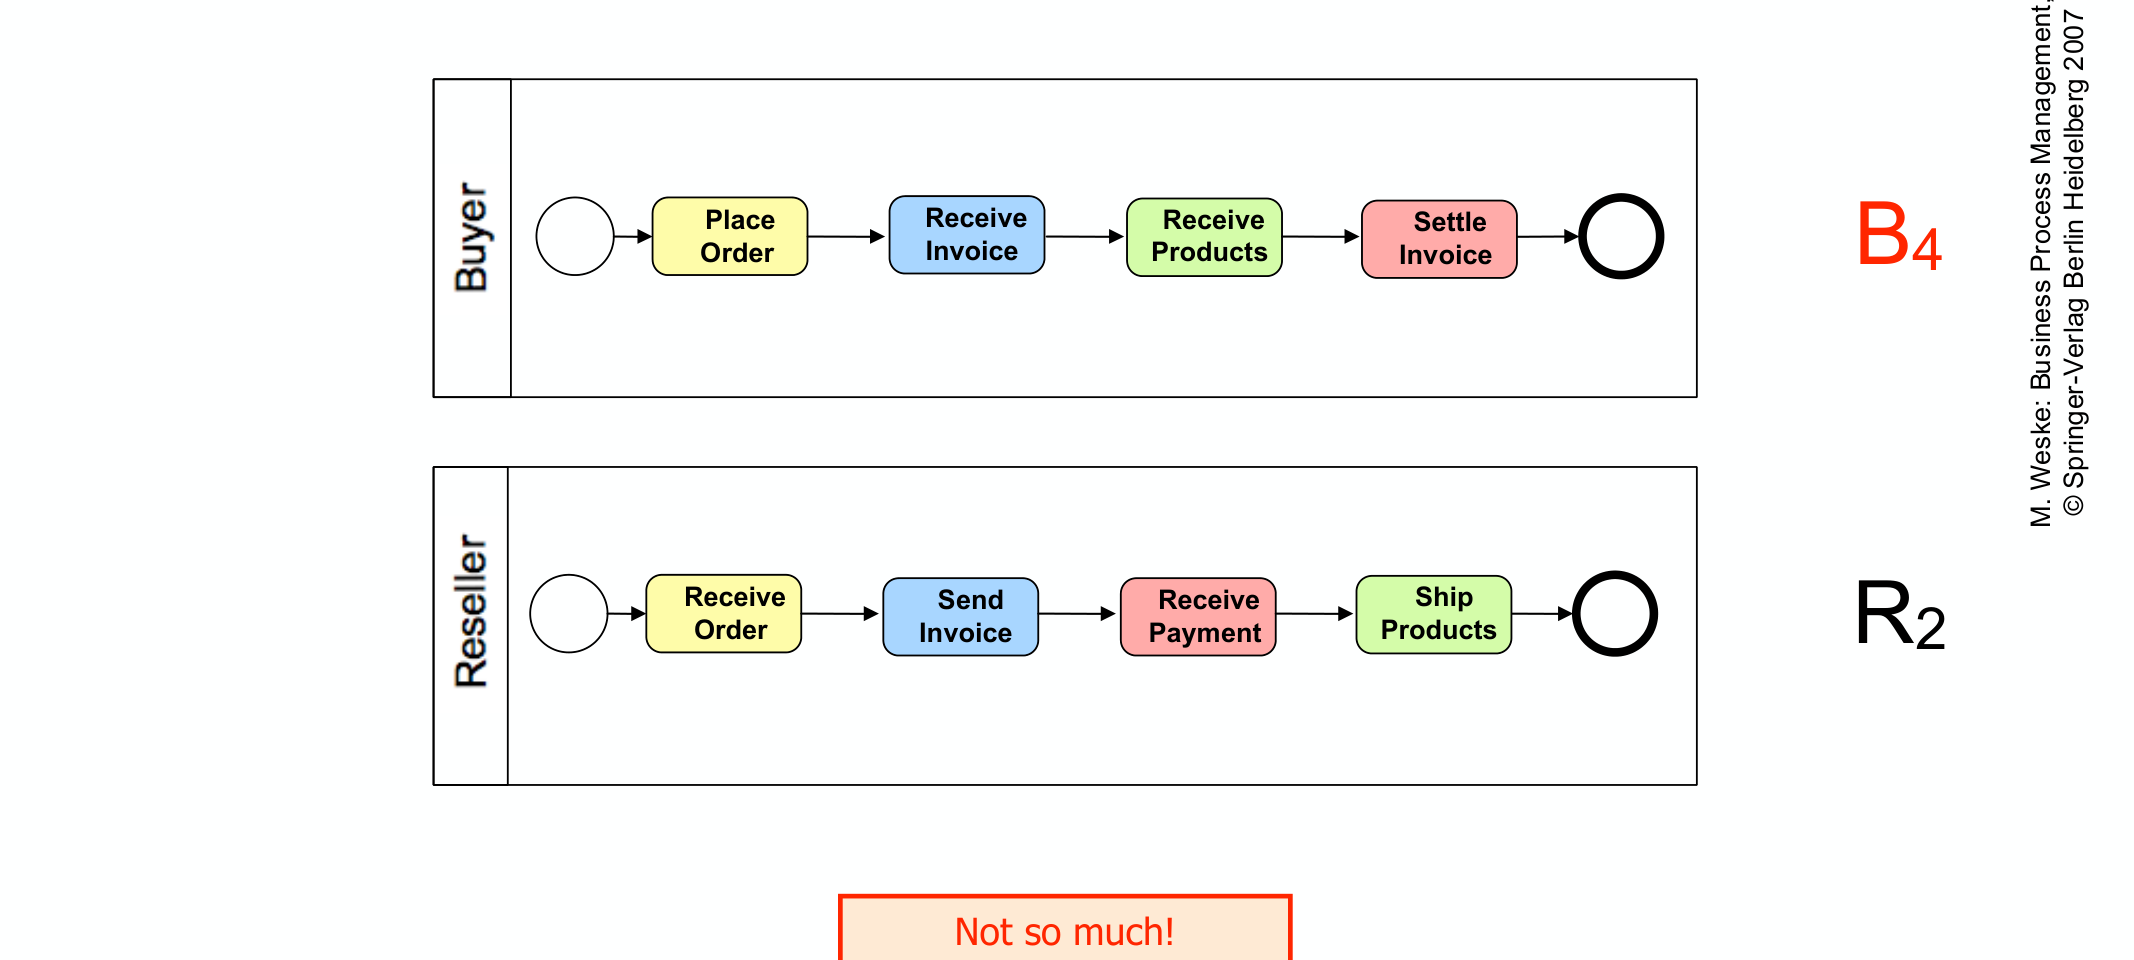
\includegraphics[width=0.74\linewidth,height=0.34\textheight,keepaspectratio]{images/06-orchestration_p46_incompatible.png}
\caption{Un'interazione \textbf{incompatibile} (B4 + R2). Si crea un \textbf{deadlock}: R2 aspetta il pagamento prima di spedire, ma B4 aspetta i prodotti prima di pagare. Nessuno dei due può proseguire, e l'interazione si blocca.}
\end{figure}

\begin{boxwarning}{Compatibilità}
Due processi sono \textbf{compatibili} se, messi a interagire, riescono a completare senza bloccarsi. Processi sviluppati in modo indipendente possono risultare \textbf{incompatibili} anche se ciascuno, preso da solo, è perfettamente corretto: il problema nasce dall'\textbf{ordine in cui si aspettano gli scambi}. Analizzando tutte le combinazioni di varianti di buyer e reseller si costruisce una \emph{compatibility matrix} che segna quali coppie funzionano ("ok") e quali no.
\end{boxwarning}

Questa nozione di "riuscire a completare senza bloccarsi" è centrale e verrà formalizzata più avanti, quando studieremo proprietà come la \textbf{soundness} delle reti. È il ponte naturale verso l'analisi strutturale dei processi. $\rightarrow$ \hyperref[ch:07a]{07 — EPC e BPMN}